% !TEX program = pdflatex
%%%%%%%%%%%%%%%%%%%%%%%%%%%%%%%%%%%%%%%%%%%%%%%%%%%%%%%%%%%%%%%%%%%%%%
%% Calibrated Bayesian Local Differential Privacy for Lightweight
%% Learning Path Recommendation
%% Springer Nature (sn-jnl) submission version, IJMLC
%%%%%%%%%%%%%%%%%%%%%%%%%%%%%%%%%%%%%%%%%%%%%%%%%%%%%%%%%%%%%%%%%%%%%%
\documentclass[pdflatex,sn-basic,Numbered]{sn-jnl}

\usepackage{graphicx}
\usepackage{multirow}
\usepackage{amsmath,amssymb,amsfonts}
\usepackage{amsthm}
\usepackage{mathrsfs}
\usepackage{xcolor}
\usepackage{booktabs}
\usepackage{algorithm}
\usepackage{algpseudocode}
\usepackage{array}
\usepackage{manyfoot}
\usepackage{url}

\graphicspath{{figures/}}

\theoremstyle{plain}
\newtheorem{theorem}{Theorem}
\newtheorem{lemma}[theorem]{Lemma}
\newtheorem{proposition}[theorem]{Proposition}
\newtheorem{corollary}[theorem]{Corollary}
\theoremstyle{remark}
\newtheorem{remark}{Remark}
\theoremstyle{definition}
\newtheorem{definition}{Definition}

\newcommand{\eps}{\varepsilon}
\newcommand{\R}{\mathbb{R}}
\newcommand{\Prob}{\Pr}
\newcommand{\logit}{\operatorname{logit}}
\newcommand{\clip}{\operatorname{clip}}
\newcommand{\E}{\mathbb{E}}
\newcommand{\Var}{\operatorname{Var}}
\newcommand{\HR}{\mathrm{HR}}
\newcommand{\NDCG}{\mathrm{NDCG}}
\providecommand{\region}[1]{#1}
\newcommand{\AUC}{\mathrm{AUC}}

\flushbottom
\renewcommand{\topfraction}{0.92}
\renewcommand{\bottomfraction}{0.5}
\renewcommand{\textfraction}{0.08}
\renewcommand{\floatpagefraction}{0.85}
\setcounter{topnumber}{3}
\setcounter{bottomnumber}{2}
\setcounter{totalnumber}{5}

\hypersetup{%
  pdftitle={Calibrated Bayesian Local Differential Privacy for Lightweight Learning Path Recommendation},
  pdfauthor={Xu Shijie, Zhai Ruiqing, Jin Xiaojuan},
  pdfkeywords={local differential privacy, randomised response, Bayesian calibration, learning path recommendation}}

% Compact reference list so that it ends on a full page.
\setlength{\bibsep}{0.55em}
\makeatletter
\def\bibfont{\reset@font\fontfamily{\rmdefault}\small\selectfont}
\makeatother

\begin{document}

\title[Calibrated Bayesian LDP for Learning Paths]{Calibrated Bayesian Local Differential Privacy for Lightweight Learning Path Recommendation}

\author[1]{\fnm{Shijie} \sur{Xu}}
\author[2]{\fnm{Ruiqing} \sur{Zhai}}
\author*[3]{\fnm{Xiaojuan} \sur{Jin}}\email{19697672@qq.com}

\affil[1,2,3]{\orgdiv{Network Center}, \orgname{Shandong Labor Vocational and Technical College}, \orgaddress{\street{Jingshi Street No.23266}, \city{Jinan}, \postcode{250014}, \region{Shandong}, \country{China}}}

\abstract{Learning path recommendation relies on student--exercise interaction logs to sequence study materials, yet raw interaction records expose sensitive knowledge states. Local differential privacy (LDP) addresses this by perturbing data on the client before transmission, though the noise introduced by randomised response (RR) typically degrades ranking quality. In this work, we present Cal-LDP-BR, a calibrated Bayesian LDP ranker. Clients upload Warner-RR reports under a tight privacy budget, after which the server reconstructs item marginals via the method of moments and ranks candidate exercises using Bayesian posterior log-odds. Because both server-side operations depend only on the released report matrix, they constitute post-processing and incur no extra privacy cost, while scoring remains linear in the candidate set without graph training. We further show that the ranking score splits exactly into a per-report evidence term of magnitude $\eps$ and an item-prior log-odds term, accounting for the non-monotone utility--budget curves observed empirically. Across ASSISTments 2009, ASSISTments 2015 and EdNet at $\eps=0.02$, Cal-LDP-BR reaches HR@10 values of 0.3907, 0.3855 and 0.4127 with membership-inference AUC scores of 0.656, 0.654 and 0.661, outperforming all evaluated $\eps$-LDP baselines on HR@10 under strict leave-last-out splitting across five fixed seeds.}

\keywords{Local differential privacy, Randomised response, Bayesian calibration, Learning path recommendation, Educational data mining, Privacy-preserving recommendation}

\maketitle

\section{Introduction}\label{sec:intro}

Online learning platforms accumulate detailed logs of student--exercise interactions, which underpin personalised learning path recommendation---ordering candidate exercises so that the next appropriate item appears near the top of the list. Although deep learning and graph neural network (GNN) recommenders capture higher-order relationships among students, exercises and knowledge points \cite{kipf2017gcn,wu2021gnnsurvey,ying2018pinsage,zhang2019survey}, deploying them in educational settings faces two practical hurdles.

Privacy is the primary concern. Interaction histories reflect a student's mastery level, error patterns and study habits, so collecting raw logs on a central server raises compliance issues under data-protection frameworks such as the GDPR and the Personal Information Protection Law (PIPL) \cite{himeur2022review}. Local differential privacy (LDP) mitigates this risk by perturbing each record on the user's device prior to upload \cite{duchi2013local,kairouz2016discrete,wang2017ldp}, removing the need for a trusted central aggregator that schools and third-party platforms seldom share across administrative boundaries.

Computational cost presents a second barrier. Multi-layer GNNs require heavy training and inference pipelines that do not fit well into the CPU-only, low-latency serving stacks typical of educational products. Simplified graph convolution (SGC) folds neighbourhood propagation into a single precomputable linear step \cite{wu2019sgc}, and LightGCN strips out feature transformations and nonlinearities \cite{he2020lightgcn}. Even so, both still rely on a graph encoder and, under LDP, must operate on a noisy adjacency matrix.

The two obstacles interact. Standard edge-level randomised response \cite{warner1965rr} on a sparse educational graph injects many false edges, and the genuine interaction signal, which is concentrated in a small fraction of the $|U|\times|P|$ cells, is overwhelmed. Recent locally private graph learning frameworks mitigate this distortion through degree-preserving perturbations \cite{hidano2024degree}, local neighbourhood augmentation \cite{pei2024privacy}, or Bayesian topology denoising with separate degree-sequence budgets for downstream GNN training \cite{zhu2023blink}. These approaches spend privacy budget on structural quantities and still train a graph encoder on a noisy adjacency.

We take a simpler approach, referred to as Cal-LDP-BR. Instead of treating perturbed bits as hard graph edges, we view single-pass Warner-RR reports as noisy observations of Bernoulli interaction indicators, recover item-conditional interaction probabilities through method-of-moments calibration, and rank candidates by their Bayesian posterior log-odds of a true interaction. This design avoids graph training and degree release in its primary form, and requires no extra privacy budget on the server because both calibration and ranking act purely as post-processing on the released report matrix.

In developing this method, we examine three issues. First, we ask whether a ranker can remain effective when the per-bit signal is well below the noise floor; Proposition 8 shows that the posterior log-odds score splits into a per-report evidence term and an item-prior term, explaining how these two components interact and why utility varies non-monotonically with the budget (Section 5.4). Second, we verify that calibration adds zero privacy cost beyond the initial report release via post-processing invariance (Theorem 1). Third, we test whether lightweight graph encoders and public skill taxonomies help on sparse educational graphs and find empirically that they hurt performance (Section 6.9).

The main contributions are summarised as follows.
\begin{enumerate}
\item We propose Cal-LDP-BR, a calibrated Bayesian LDP ranker that reconstructs item-conditional interaction probabilities from Warner-RR reports and ranks candidate exercises by posterior log-odds (Sections~\ref{sec:method}--\ref{sec:theory}). The moment estimator is unbiased before clipping, its variance is available in closed form, and the ranking rule is Bayes-optimal under the RR likelihood.
\item We give a complete privacy treatment: standard Warner RR establishes the exact $\eps$-LDP guarantee of the primary method, while sampling amplification and private degree release are analysed as an optional adaptive variant with explicit composition accounting (Theorem~\ref{thm:privacy} and Lemma~\ref{lem:amplification}).
\item We derive an exact decomposition of the ranking score into evidence and prior components, and use it to explain the non-monotone utility--budget behaviour that LDP rankers exhibit under leave-last-out evaluation (Proposition~\ref{prop:decomposition}, Section~\ref{sec:regimes}).
\item We investigate a lightweight SGC alternative with soft posterior weights and a public skill graph; ablation studies show that neither component improves utility on the tested sparse educational graphs, and the negative results are retained (Section~\ref{sec:ablation}).
\item We conduct a reproducible evaluation under strict leave-last-out splitting across five fixed seeds, including paired $t$-tests, Wilcoxon signed-rank tests with exact attainable $p$-values, 95\% confidence intervals for paired differences, full $\eps$-sensitivity sweeps, a full-population validation, and public release of code and processing scripts (Section~\ref{sec:experiments}).
\end{enumerate}

The remainder of the paper is organised as follows. Section~\ref{sec:related} reviews related work. Section~\ref{sec:prelim} introduces preliminaries and the problem formulation. Section~\ref{sec:method} presents Cal-LDP-BR, the optional adaptive variant and the lightweight SGC variant. Section~\ref{sec:theory} provides the privacy and utility analysis. Section~\ref{sec:experiments} reports experimental results, statistical tests and sensitivity analyses. Section~\ref{sec:discussion} discusses implications and threats to validity, and Section~\ref{sec:conclusion} concludes.

\section{Related work}\label{sec:related}

\subsection{Learning path recommendation and knowledge tracing}

Existing learning path recommenders fall broadly into knowledge-tracing, sequence-based and graph-based families. Deep knowledge tracing (DKT) models track temporal skill mastery from exercise sequences \cite{piech2015dkt}, while exercise-aware extensions incorporate exercise metadata into the hidden state \cite{liu2021ekt}. Graph-based methods build student--exercise or multi-source interaction graphs and employ encoders such as GCN \cite{kipf2017gcn}, PinSage \cite{ying2018pinsage}, NGCF \cite{wang2019ngcf} and multi-source fusion architectures \cite{cheng2019friend} to capture collaborative and structural patterns \cite{wu2021gnnsurvey,zhang2019survey}, with graph-based knowledge tracing applying similar encoders to skill graphs \cite{nakagawa2019gkt}. Knowledge-graph-based models further encode multidimensional semantic relations \cite{shi2020learningpath}, while a comprehensive survey of learning path personalisation highlights the prevalence of sequence models alongside the lack of formal privacy guarantees in deployed systems \cite{nabizadeh2020survey}.

Educational interaction logs exhibit two characteristics that strongly influence model design. Interaction matrices are typically very sparse---a student usually completes tens or hundreds of exercises out of thousands---making collaborative filtering signals weak and item popularity a surprisingly competitive baseline. In addition, the natural evaluation setting is leave-last-out rather than random missing-entry imputation, since the practical goal is predicting the next exercise. Because both properties interact with privacy noise in ways obscured by random splits, we enforce a strict leave-last-out protocol throughout (Section 6.2).

\subsection{Differential privacy and local differential privacy}

Differential privacy (DP) provides rigorous guarantees against individual record inference \cite{dwork2006calibrating,dwork2014algorithmic}. In recommender systems, DP has been applied to matrix factorisation \cite{mcsherry2009dp,ran2022dpnmf} and to privacy-preserving frameworks reviewed in \cite{himeur2022review}. These approaches assume a trusted curator that holds the raw data.

LDP avoids the trusted-curator assumption by perturbing user records locally on the client \cite{duchi2013local,kairouz2016discrete,kasiviswanathan2011private}. Warner's randomised response provides the foundational binary mechanism \cite{warner1965rr}, which large-scale systems like RAPPOR \cite{erlingsson2014rappor} and frequency-estimation protocols \cite{bassily2015local,cormode2018frequency,wang2017ldp} extend to categorical and ordinal data. On graphs, LDP has been used for topology and metric estimation \cite{ye2022lfgdpr}, degree-preserving randomised response \cite{hidano2024degree}, local graph augmentation defending against attribute and link-stealing attacks \cite{pei2024privacy}, and Bayesian link denoising for GNN training \cite{zhu2023blink}. More recently, Bayesian reconstruction from RR reports has been applied to implicit-feedback recommendation \cite{tang2025bayesian}. Our work adapts this direction to educational learning paths without graph training or mandatory degree budgets, while evaluating both formal privacy budgets and empirical membership-inference leakage.

\subsection{Privacy amplification, composition and empirical leakage}

Sampling amplification and sequential composition are the standard tools for converting per-record budgets into end-to-end guarantees \cite{kasiviswanathan2011private,dwork2014algorithmic,balle2018amplification}. Because formal guarantees are necessary but not sufficient for user trust, empirical leakage is increasingly reported alongside the budget. Membership-inference attacks \cite{shokri2017mia} and their likelihood-ratio refinements \cite{carlini2022mia} provide a reproducible way to measure whether a released artefact reveals whether a particular record was used. We report both the theoretical budget and an empirical membership-inference AUC.

\subsection{Lightweight graph convolution}

LightGCN simplifies graph collaborative filtering by removing feature transformations and nonlinear activations \cite{he2020lightgcn}, while SGC further precomputes $K$-order propagation into a single linear smoothing step \cite{wu2019sgc}. Lightweight graph encoders are rarely combined with formal local privacy guarantees in educational settings. We examine whether SGC over calibrated soft graphs offers gains over direct posterior ranking, and we report the outcome either way.

Table~\ref{tab:related} positions Cal-LDP-BR against the closest locally private graph learning approaches.

\begin{table}[t]
\caption{Positioning against locally private graph learning approaches.}
\label{tab:related}
\footnotesize
\setlength{\tabcolsep}{1.5pt}
\begin{tabular}{@{}lcccccc@{}}
\toprule
Approach & Perturbation & Graph enc. & Degree $\eps$ & Bayes.\ calib. & Sparse educ. & CPU serving \\
\midrule
Edge RR + GCN \cite{sajadmanesh2021lpgnn} & edge RR & yes & no & no & partial & no \\
Degree-pres.\ RR \cite{hidano2024degree} & degree-aware RR & yes & implicit & no & no & no \\
Local augmentation \cite{pei2024privacy} & edge RR & yes & no & no & no & no \\
Blink \cite{zhu2023blink} & edge RR & yes & yes & yes & no & no \\
Bayesian LDP rec.\ \cite{tang2025bayesian} & item RR & no & no & yes & no & yes \\
\textbf{Cal-LDP-BR} (this work) & Warner RR & no & optional & yes & yes & yes \\
\bottomrule
\end{tabular}

\vspace{2pt}
{\footnotesize ``Graph enc.''\ denotes an iterative encoder trained on a noisy adjacency; ``degree $\eps$''\ denotes budget spent on releasing degree information; ``Bayes.\ calib.''\ denotes explicit reconstruction of interaction probabilities from RR reports; ``sparse educ.''\ denotes evaluation on educational interaction graphs with leave-last-out protocols.}
\end{table}

\section{Preliminaries and problem formulation}\label{sec:prelim}

\subsection{Notation}

Table~\ref{tab:notation} collects the notation used throughout. Vectors are column vectors and $\mathbf{1}[\cdot]$ denotes the indicator function.

\begin{table}[t]
\caption{Notation.}
\label{tab:notation}
\small
\begin{tabular}{@{}ll@{}}
\toprule
Symbol & Meaning \\
\midrule
$U$, $P$ & sets of students and exercises, $n=|U|$, $m=|P|$ \\
$R\in\{0,1\}^{n\times m}$ & binary interaction matrix, $R_{u,i}=1$ if student $u$ interacted with exercise $i$ \\
$x_{u}\in\{0,1\}^{m}$ & interaction vector of student $u$ (a row of $R$) \\
$d_u=\sum_i x_{u,i}$ & number of interactions of student $u$ \\
$\eps$ & local privacy budget \\
$p$, $q$ & RR true-positive and false-positive reporting probabilities, Eq.~\eqref{eq:rr} \\
$A\in\{0,1\}^{n\times m}$ & released report matrix, $A_{u,i}$ is the reported bit \\
$\bar a_i$ & empirical reporting rate of exercise $i$, $\bar a_i=n^{-1}\sum_u A_{u,i}$ \\
$\pi_i$ & true marginal $\Prob[x_{u,i}=1]$ for a randomly drawn student \\
$\hat\pi_i$ & calibrated (method-of-moments) estimate of $\pi_i$ \\
$\gamma_u$ & per-student sampling rate of the adaptive variant \\
$s_{u,i}$ & posterior log-odds score of exercise $i$ for student $u$ \\
$\mathcal{N}_u$ & candidate set of student $u$ (one positive, $|\mathcal{N}_u|-1$ negatives) \\
$K$ & truncation depth of the recommendation list ($K=10$ in experiments) \\
$S$ & symmetrically normalised adjacency with self-loops \\
$\lambda$ & weight of the public skill graph in the SGC variant \\
\bottomrule
\end{tabular}
\end{table}

\subsection{Local differential privacy}

\begin{definition}[$\eps$-LDP]\label{def:ldp}
A randomised mechanism $\mathcal{M}$ satisfies $\eps$-local differential privacy if, for any pair of neighbouring local records $x,x'\in\{0,1\}^{m}$ differing in one coordinate and any measurable output $y$ in the range of $\mathcal{M}$,
\begin{equation}\label{eq:ldp}
\Prob[\mathcal{M}(x)=y]\le e^{\eps}\,\Prob[\mathcal{M}(x')=y].
\end{equation}
\end{definition}

A smaller budget $\eps>0$ enforces stronger indistinguishability. Two composition properties are used below. \emph{Parallel composition} states that mechanisms applied to disjoint subsets of a user's coordinates compose without budget growth. \emph{Post-processing} states that any deterministic or randomised function of a private output remains private with the same budget \cite{dwork2014algorithmic}.

\begin{definition}[Warner randomised response]\label{def:rr}
For a binary record $x\in\{0,1\}$, Warner RR releases
\begin{equation}\label{eq:rr}
a=\begin{cases} x & \text{with probability } p=\dfrac{e^{\eps}}{1+e^{\eps}},\\[2mm] 1-x & \text{with probability } q=\dfrac{1}{1+e^{\eps}}.\end{cases}
\end{equation}
\end{definition}

The mechanism satisfies $\eps$-LDP exactly, since $p/q=e^{\eps}$ and $(1-q)/(1-p)=e^{\eps}$ \cite{warner1965rr,dwork2014algorithmic}. Two derived quantities recur: the \emph{signal} $p-q=\tanh(\eps/2)$ and the \emph{noise floor} $q=1/(1+e^{\eps})$. At $\eps=0.02$, $p=0.5050$, $q=0.4950$ and $p-q\approx0.01$: each reported bit carries little more than one per cent of information about the underlying interaction.

\subsection{Simplified graph convolution}

Given an interaction matrix $R$, let $S$ denote the symmetrically normalised adjacency of the student--exercise bipartite graph with self-loops. SGC computes $K$-step smoothed embeddings $Z=S^{K}X$ by iterative sparse--dense multiplication without materialising $S^{K}$ \cite{wu2019sgc}. The cost of one propagation step is $O(\mathrm{nnz}(S)\,d)$ for embedding dimension $d$.

\subsection{Problem formulation}\label{sec:problem}

Let $\mathcal{N}_u\subseteq P$ be the candidate set of student $u$, containing the item to be predicted and a set of negatives. A recommender outputs a ranking $\sigma_u$ of $\mathcal{N}_u$. We write $\HR@K$ and $\NDCG@K$ for the hit rate and normalised discounted cumulative gain at cutoff $K$, defined in Section~\ref{sec:metrics}. The design problem is
\begin{equation}\label{eq:problem}
\begin{aligned}
\max_{\sigma}\;\; & \E_{u}\big[\HR@K(\sigma_u)\big]\\
\text{s.t.}\;\; & \text{(i) every released record satisfies $\eps$-LDP;}\\
& \text{(ii) scoring runs on CPU in time } O(|\mathcal{N}_u|).
\end{aligned}
\end{equation}
Condition (ii) excludes iterative graph training at serving time. A secondary goal is to incorporate a public skill taxonomy $G_{\text{skill}}$ when it improves utility; Section~\ref{sec:ablation} shows that on the tested graphs it does not.

\section{Proposed method}\label{sec:method}

\subsection{Overview}

Figure~\ref{fig:framework} summarises the protocol. The client perturbs every interaction bit with Warner RR and uploads only the resulting bit vector. The server performs two operations on the collected report matrix: it estimates each item marginal by the method of moments (Section~\ref{sec:calibration}), and it scores candidate exercises by the posterior log-odds of a true interaction given the report and the estimated marginal (Section~\ref{sec:ranking}). Both server-side operations are functions of the released matrix alone and therefore consume no additional privacy budget (Theorem~\ref{thm:privacy}). Algorithm~\ref{alg:calldpbr} states the protocol and attaches the privacy accounting to each stage.

\begin{figure}[t]
\centering
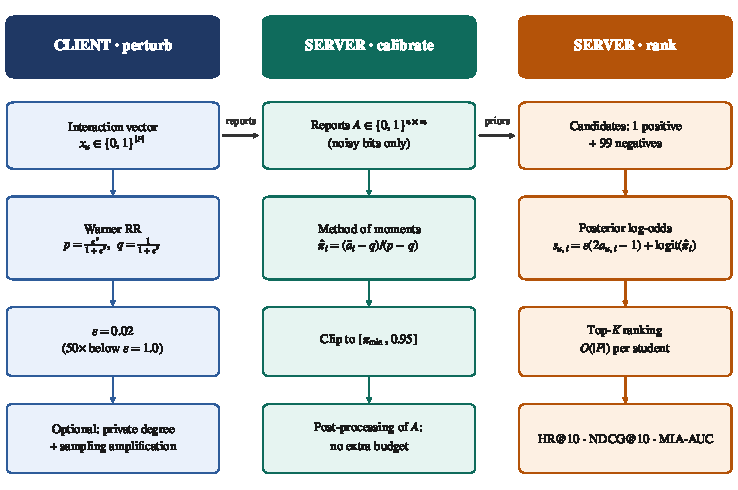
\includegraphics[width=\textwidth]{fig1_framework.pdf}
\caption{Overall framework of Cal-LDP-BR. The client perturbs each interaction locally under $\eps$-LDP; the server calibrates item marginals from the released reports and ranks candidates by Bayesian posterior log-odds. Both server steps are post-processing of released data and consume no additional privacy budget (Theorem~\ref{thm:privacy}).}
\label{fig:framework}
\end{figure}

Three properties follow from the construction and are made precise in Section~\ref{sec:theory}: (i) calibration recovers a rank-consistent item signal from heavily perturbed reports, because the moment estimator is an affine function of the reported rate; (ii) the ranking score is the Bayes-optimal posterior log-odds under the RR likelihood, so the noise channel is exploited statistically rather than treated as a hard graph edge; and (iii) privacy is guaranteed end-to-end at the client, while all server-side operations are post-processing.

\subsection{Client-side local perturbation}\label{sec:client}

In the primary protocol, each student $u$ applies Warner RR, Eq.~\eqref{eq:rr}, independently to every exercise bit $x_{u,i}$. Because the coordinates are disjoint binary indicators, parallel composition yields exact $\eps$-LDP for the student's full interaction vector:
\begin{equation}\label{eq:vector}
\Prob[A_{u}=a\mid x_u]=\prod_{i=1}^{m}\Prob[a_i\mid x_{u,i}],\qquad
\frac{\Prob[A_u=a\mid x_u]}{\Prob[A_u=a\mid x'_u]}\le e^{\eps}.
\end{equation}
We adopt $\eps=0.02$ as the default operating point and evaluate sensitivity across $\eps\in[0.005,2]$ in Section~\ref{sec:sweep}.

As an optional degree-adaptive variant (Section~\ref{sec:adaptive}), the student first releases a Laplace-perturbed degree $\tilde d_u=d_u+\mathrm{Lap}(1/\eps_0)$ under budget $\eps_0$, and sets the sampling rate
\begin{equation}\label{eq:gamma}
\gamma_u=\clip\!\left(\left(\frac{d_{\text{ref}}}{\tilde d_u}\right)^{\eta},\gamma_{\min},\gamma_{\max}\right),
\end{equation}
where $d_{\text{ref}}$ is a public reference degree and $\eta\in[0,1]$ controls the strength of the adjustment. Coordinates are then sub-sampled with probability $\gamma_u$ before RR, which yields the per-user budget $\ln\!\big(1+\gamma_u(e^{\eps_{\text{int}}}-1)\big)$ by Lemma~\ref{lem:amplification}.

\subsection{Item-wise calibration}\label{sec:calibration}

Let $a_{u,i}\in\{0,1\}$ denote the reported bit for student $u$ and exercise $i$. From the released matrix $A$, the server estimates the true item marginal $\pi_i=\Prob[x_{u,i}=1]$ by the method of moments:
\begin{equation}\label{eq:pihat}
\hat\pi_i=\frac{\bar a_i-q}{p-q},\qquad \bar a_i=\frac{1}{n}\sum_{u=1}^{n}a_{u,i},
\end{equation}
which is unbiased before clipping, $\E[\hat\pi_i]=\pi_i$ (Theorem~\ref{thm:unbiased}). Because the estimate can leave the probability simplex when $p-q$ is small, it is clipped to a bounded interval:
\begin{equation}\label{eq:clip}
\hat\pi_i^{c}=\min\{\max\{\hat\pi_i,\pi_{\min}\},\,0.95\},
\end{equation}
with $\pi_{\min}\ge 0$. The upper bound prevents a single high-report item from dominating the prior term, and the lower bound removes negative estimates. The clipped estimator is biased by construction; Proposition~\ref{prop:clipping} bounds the bias. For the adaptive variant, the estimator generalises to the $\gamma_u$-weighted form
\begin{equation}\label{eq:pihat-adaptive}
\hat\pi_i=\frac{\sum_u a_{u,i}-q\sum_u\gamma_u}{(p-q)\sum_u\gamma_u},
\end{equation}
which reduces to Eq.~\eqref{eq:pihat} when $\gamma_u\equiv1$.

Because $\hat\pi_i$ is computed solely from the published matrix $A$, it constitutes post-processing and consumes zero additional privacy budget. The calibration is also inexpensive: one pass over the reported entries, $O(\mathrm{nnz}(A))$ time and $O(m)$ memory.

\subsection{Bayesian posterior ranking}\label{sec:ranking}

For a candidate exercise $i$, the server observes the student's report $a_{u,i}$ and holds the estimated marginal $\hat\pi_i$. Treating the report as a draw from the RR channel with a Bernoulli prior $\Prob[x_{u,i}=1]=\hat\pi_i$, the posterior log-odds of a true interaction is
\begin{equation}\label{eq:score}
s_{u,i}=\begin{cases}
\log\dfrac{p\,\hat\pi_i}{q\,(1-\hat\pi_i)}, & a_{u,i}=1,\\[3mm]
\log\dfrac{(1-p)\,\hat\pi_i}{(1-q)\,(1-\hat\pi_i)}, & a_{u,i}=0.
\end{cases}
\end{equation}
Candidates are ranked in descending order of $s_{u,i}$, and the top-$K$ list is returned. The rule is Bayes-optimal for binary relevance under the assumed likelihood (Theorem~\ref{thm:bayes}), and it costs $O(1)$ arithmetic per candidate, i.e.\ $O(|\mathcal{N}_u|)$ per student.

Equation~\eqref{eq:score} has a compact form that drives the analysis of Section~\ref{sec:regimes}. Since $\log(p/q)=\eps$ and $\log\big((1-p)/(1-q)\big)=-\eps$, both branches collapse to
\begin{equation}\label{eq:decomposition}
s_{u,i}=\eps\,(2a_{u,i}-1)+\logit(\hat\pi_i),\qquad \logit(\pi)=\log\frac{\pi}{1-\pi}.
\end{equation}
The score is therefore the sum of an \emph{evidence} term, which equals $+\eps$ for a reported interaction and $-\eps$ for a reported non-interaction, and an \emph{item-prior} term, which is shared by all students. The relative weight of the two terms is governed by $\eps$ alone, which explains why the utility--budget curve is not monotone (Section~\ref{sec:regimes}).

\subsection{Optional degree-adaptive variant}\label{sec:adaptive}

Sparse students contribute few positive bits and many negative ones, so a uniform reporting rate spends most of the budget on uninformative coordinates. The adaptive variant scales the sampling rate with the privately released degree, Eq.~\eqref{eq:gamma}, so that active students are sub-sampled more aggressively and inactive students report more of their (mostly negative) coordinates. Privacy accounting combines the Laplace mechanism for the degree, sampling amplification for the sub-sampled RR, and sequential composition:
\begin{equation}\label{eq:budget}
\eps_{\text{tot}}\le\eps_0+\max_{u}\ln\!\big(1+\gamma_u(e^{\eps_{\text{int}}}-1)\big)\le\eps,
\end{equation}
which is verified numerically for every user in our implementation. Algorithm~\ref{alg:adaptive} summarises the variant; Section~\ref{sec:ablation} reports its empirical behaviour.

\subsection{Lightweight SGC variant}\label{sec:sgc}

For comparison we also evaluate a lightweight SGC encoder trained on the calibrated soft posterior graph $R'$, whose entries are the posterior probabilities implied by Eq.~\eqref{eq:score}, mapped to $[0,1]$. Public skill taxonomy edges $G_{\text{skill}}$ connect exercises that share a knowledge point and are fused through the normalised block adjacency
\begin{equation}\label{eq:blockadj}
S=\operatorname{norm}\!\left(\begin{bmatrix}0 & R'\\ R'^{\top} & \lambda\,G_{\text{skill}}\end{bmatrix}\right),
\end{equation}
with propagation
\begin{equation}\label{eq:sgc}
Z=S^{K}X,\qquad K=3,
\end{equation}
where $X$ stacks free student and exercise embeddings of dimension $d=64$, and $\lambda=0.3$ weights the skill edges. Each propagation step costs $O(\mathrm{nnz}(S)\,d)$. Section~\ref{sec:ablation} shows that adding SGC and the skill graph degrades accuracy on sparse educational graphs; the direct posterior ranker therefore remains the primary method, and the negative ablation results are retained.

\subsection{Complexity and deployment}\label{sec:complexity}

Table~\ref{tab:complexity} compares the asymptotic costs of the evaluated families. Cal-LDP-BR has no training phase, no parameters, and a per-student scoring cost linear in the candidate set, which makes it suitable for CPU-only serving. The SGC variant adds a precomputable propagation but requires materialising soft edges and a skill graph; the GNN baselines require iterative training over the noisy graph.

\begin{table}[t]
\caption{Asymptotic cost of the evaluated method families. $n=|U|$, $m=|P|$, $d$ is the embedding dimension, $K$ the propagation depth, $T$ the number of training epochs, and $\mathrm{nnz}(\cdot)$ the number of non-zeros. Costs are per epoch for trained models and per scoring pass for Cal-LDP-BR.}
\label{tab:complexity}
\footnotesize
\setlength{\tabcolsep}{3.5pt}
\begin{tabular}{@{}lcccc@{}}
\toprule
Method & Training & Inference / student & Parameters & Extra budget \\
\midrule
Cal-LDP-BR & none & $O(|\mathcal{N}_u|)$ & $0$ & none \\
Adaptive-LDP-SGC-LP & $O(TK\,\mathrm{nnz}(S)d)$ & $O(K\,\mathrm{nnz}(S_{\cdot,u})d)$ & $(n+m)d$ & $\eps_0$ \\
LDP-GCN, LDP-RR-Light & $O(T\,\mathrm{nnz}(A)d)$ & $O(\mathrm{nnz}(A_{\cdot,u})d)$ & $(n+m)d$ & none \\
GCN-LP, LightGCN-LP & $O(T\,\mathrm{nnz}(R)d)$ & $O(\mathrm{nnz}(R_{\cdot,u})d)$ & $(n+m)d$ & not private \\
\bottomrule
\end{tabular}
\end{table}

\begin{algorithm}[t]
\caption{Cal-LDP-BR: client--server protocol with privacy accounting.}\label{alg:calldpbr}
\begin{algorithmic}[1]
\Require interaction vectors $\{x_u\}_{u\in U}$, budget $\eps$, clip bounds $\pi_{\min}$, $\pi_{\max}=0.95$, cutoff $K$
\Statex \textbf{Client side} (executed on device; one pass)
\For{each student $u$ and exercise $i$}
  \State draw $a_{u,i}\gets x_{u,i}$ with probability $p=e^{\eps}/(1+e^{\eps})$, else $1-x_{u,i}$ \Comment{Eq.~\eqref{eq:rr}}
\EndFor
\State upload $a_u\in\{0,1\}^m$ only \Comment{$\eps$-LDP by parallel composition, Theorem~\ref{thm:privacy}}
\Statex \textbf{Server side} (post-processing; no budget)
\State form the report matrix $A=[a_1,\dots,a_n]^{\top}$
\For{each exercise $i$}
  \State $\bar a_i\gets n^{-1}\sum_u a_{u,i}$; \quad $\hat\pi_i\gets(\bar a_i-q)/(p-q)$ \Comment{Eq.~\eqref{eq:pihat}}
  \State $\hat\pi_i^{c}\gets\min\{\max\{\hat\pi_i,\pi_{\min}\},\pi_{\max}\}$ \Comment{Eq.~\eqref{eq:clip}}
\EndFor
\For{each student $u$}
  \For{each candidate $i\in\mathcal{N}_u$}
    \State $s_{u,i}\gets \eps(2a_{u,i}-1)+\logit(\hat\pi_i^{c})$ \Comment{Eqs.~\eqref{eq:score}, \eqref{eq:decomposition}}
  \EndFor
  \State return the $K$ candidates with largest $s_{u,i}$
\EndFor
\end{algorithmic}
\end{algorithm}

\begin{algorithm}[t]
\caption{Degree-adaptive sampling-amplified variant (optional).}\label{alg:adaptive}
\begin{algorithmic}[1]
\Require budget $\eps$, split $\eps_0+\eps_{\text{int}}=\eps$, reference degree $d_{\text{ref}}$, exponent $\eta$, bounds $\gamma_{\min},\gamma_{\max}$
\Statex \textbf{Client side}
\State $d_u\gets\sum_i x_{u,i}$;\quad $\tilde d_u\gets d_u+\mathrm{Lap}(1/\eps_0)$ \Comment{$\eps_0$-DP}
\State $\gamma_u\gets\clip((d_{\text{ref}}/\tilde d_u)^{\eta},\gamma_{\min},\gamma_{\max})$ \Comment{Eq.~\eqref{eq:gamma}}
\For{each exercise $i$}
  \State sample $b_i\sim\mathrm{Bernoulli}(\gamma_u)$; \State if $b_i=1$ release $a_{u,i}\sim\mathrm{RR}_{\eps_{\text{int}}}(x_{u,i})$, else release nothing
\EndFor
\Statex \textbf{Server side}
\State estimate $\hat\pi_i$ by Eq.~\eqref{eq:pihat-adaptive} using the observed $\gamma_u$
\State rank by Eq.~\eqref{eq:score} with the effective probabilities $\gamma_u p$ and $\gamma_u q$
\end{algorithmic}
\end{algorithm}

\section{Theoretical analysis}\label{sec:theory}

This section establishes the privacy guarantee of the protocol (Section~\ref{sec:privacy-theory}), the statistical properties of the calibrated estimator (Section~\ref{sec:utility-theory}), the optimality of the ranking rule (Section~\ref{sec:bayes}), and the consequences of the score decomposition for the operating regime (Section~\ref{sec:regimes}). Proofs are given in place where short and in Appendix~\ref{app:proofs} where they are technical.

\subsection{Privacy guarantees}\label{sec:privacy-theory}

\begin{theorem}[Privacy of the primary protocol]\label{thm:privacy}
Warner RR with $p/q=e^{\eps}$ and $(1-q)/(1-p)=e^{\eps}$ satisfies exact $\eps$-LDP for each interaction bit. Applying it independently across the $m$ disjoint exercise coordinates preserves the $\eps$-LDP bound for the student's entire interaction vector by parallel composition. Item-marginal estimation, clipping and posterior log-odds ranking operate strictly on the released report matrix $A$ and therefore incur no additional privacy loss.
\end{theorem}

\begin{proof}
Fix a student and two neighbouring vectors $x,x'\in\{0,1\}^{m}$ that differ in coordinate $j$. For any report vector $a\in\{0,1\}^{m}$,
\begin{equation}\label{eq:proof-ratio}
\frac{\Prob[A=a\mid x]}{\Prob[A=a\mid x']}
=\prod_{i=1}^{m}\frac{\Prob[a_i\mid x_i]}{\Prob[a_i\mid x'_i]}
=\frac{\Prob[a_j\mid x_j]}{\Prob[a_j\mid x'_j]},
\end{equation}
because all other factors equal one. If $x_j=1$ and $x'_j=0$, the ratio equals $p/q=e^{\eps}$ when $a_j=1$ and $(1-p)/(1-q)=e^{\eps}$ when $a_j=0$. The reversed case is symmetric. Hence the ratio is at most $e^{\eps}$, which is Eq.~\eqref{eq:ldp} for the vector mechanism. Post-processing invariance \cite{dwork2014algorithmic} applies to $\hat\pi$, $\hat\pi^{c}$ and $s$, each of which is a function of $A$ alone.
\end{proof}

\begin{lemma}[Sampling amplification]\label{lem:amplification}
Let $\mathcal{M}$ be an $\eps_{\text{int}}$-LDP mechanism on interaction vectors, and let $S_\gamma$ retain each coordinate independently with probability $\gamma$. Under add/remove adjacency, the composed mechanism $\mathcal{M}\circ S_\gamma$ satisfies $\eps'$-LDP with
\begin{equation}\label{eq:amplification}
\eps'=\ln\!\big(1+\gamma(e^{\eps_{\text{int}}}-1)\big)\le\gamma\,\eps_{\text{int}}.
\end{equation}
\end{lemma}

\begin{proof}
Let $x$ contain the differing coordinate and $x'$ be $x$ with that coordinate removed. Condition on the sampling set $S$. If the differing coordinate is absent from $S$, which happens with probability $1-\gamma$, then $S_\gamma(x)$ and $S_\gamma(x')$ coincide, so the two output distributions are identical and contribute a common mixture component $\mu$. With probability $\gamma$ the coordinate is retained and the two sampled vectors are add/remove neighbours, so the conditional distributions $\nu$ and $\mu$ satisfy $\nu\le e^{\eps_{\text{int}}}\mu$ pointwise by $\eps_{\text{int}}$-LDP. Therefore, for every output $y$,
\begin{equation}
\begin{aligned}
\Prob[\mathcal{M}(S_\gamma(x))=y]&=(1-\gamma)\mu(y)+\gamma\nu(y)\\
&\le\big(1+\gamma(e^{\eps_{\text{int}}}-1)\big)\mu(y)
=e^{\eps'}\Prob[\mathcal{M}(S_\gamma(x'))=y],
\end{aligned}
\end{equation}
which is the claim. The inequality $\ln(1+\gamma(e^{\eps}-1))\le\gamma\eps$ follows from concavity of the logarithm, so the amplified budget never exceeds the linear interpolation between $0$ and $\eps$.
\end{proof}

\begin{corollary}[Budget of the adaptive variant]\label{cor:budget}
Releasing $\tilde d_u=d_u+\mathrm{Lap}(1/\eps_0)$ satisfies $\eps_0$-DP, and $\gamma_u$ is a post-processing function of $\tilde d_u$. By sequential composition, the total per-user budget of Algorithm~\ref{alg:adaptive} is at most
\begin{equation}\label{eq:totalbudget}
\eps_{\text{tot}}\le\eps_0+\max_{u}\ln\!\big(1+\gamma_u(e^{\eps_{\text{int}}}-1)\big)\le\eps .
\end{equation}
\end{corollary}

\begin{proof}
The Laplace mechanism with scale $1/\eps_0$ is $\eps_0$-DP for a sensitivity-one degree query \cite{dwork2006calibrating}. The sampling rate is a deterministic function of the noisy degree and hence post-processing. Lemma~\ref{lem:amplification} bounds the RR component for each user, and sequential composition over the two releases gives Eq.~\eqref{eq:totalbudget}. Our implementation evaluates the right-hand side for every user and rejects configurations that violate the cap.
\end{proof}

\subsection{Unbiasedness, variance and clipping}\label{sec:utility-theory}

\begin{theorem}[Unbiasedness of the moment estimator]\label{thm:unbiased}
Let $a_{u,i}$ be a reported cell with effective reporting probabilities $p_u=\gamma_u p$ and $q_u=\gamma_u q$, where $\gamma_u\equiv1$ for the uniform protocol. The inverse-probability estimator
\begin{equation}\label{eq:xhat}
\hat x_{u,i}=\frac{a_{u,i}-q_u}{p_u-q_u}
\end{equation}
is unbiased for the true indicator $x_{u,i}$, and its variance is
\begin{equation}\label{eq:varx}
\Var(\hat x_{u,i})=\frac{\theta_{u,i}(1-\theta_{u,i})}{(p_u-q_u)^{2}},
\qquad \theta_{u,i}=q_u+x_{u,i}(p_u-q_u).
\end{equation}
Consequently the aggregated estimator of Eq.~\eqref{eq:pihat} is unbiased for $\pi_i$ before clipping.
\end{theorem}

\begin{proof}
Since $a_{u,i}$ is Bernoulli with mean $\theta_{u,i}=q_u+x_{u,i}(p_u-q_u)$, linearity gives $\E[\hat x_{u,i}]=(q_u+x_{u,i}(p_u-q_u)-q_u)/(p_u-q_u)=x_{u,i}$. The variance follows from $\Var(a)=\theta(1-\theta)$ and the scaling by $(p_u-q_u)^{-2}$. Averaging $\hat x_{u,i}$ over $u$ and using linearity of expectation yields $\E[\hat\pi_i]=\pi_i$; for the weighted form of Eq.~\eqref{eq:pihat-adaptive} the same argument applies with weights $\gamma_u/\sum_v\gamma_v$.
\end{proof}

\begin{corollary}[Standard error and sample-size requirement]\label{cor:se}
For the uniform protocol the standard error of $\hat\pi_i$ satisfies
\begin{equation}\label{eq:se}
\mathrm{SE}(\hat\pi_i)\le\frac{1}{2\,(p-q)\sqrt{n}}=\frac{1}{2\tanh(\eps/2)\sqrt{n}} ,
\end{equation}
with equality in the worst case $\pi_i=1/2$. Reaching a target standard error $\tau$ therefore requires
\begin{equation}\label{eq:nreq}
n\ \ge\ \frac{1}{4\,\tau^{2}\,(p-q)^{2}} .
\end{equation}
\end{corollary}

\begin{proof}
The estimator is a sample mean of independent terms scaled by $(p-q)^{-1}$, so $\Var(\hat\pi_i)=n^{-1}\sum_u\theta_u(1-\theta_u)/(p-q)^{2}\le 1/(4n(p-q)^{2})$ because $\theta(1-\theta)\le1/4$. Taking square roots gives Eq.~\eqref{eq:se}; solving for $n$ gives Eq.~\eqref{eq:nreq}.
\end{proof}

\begin{proposition}[Bias introduced by clipping]\label{prop:clipping}
Let $\hat\pi^{c}$ be the clipped estimator of Eq.~\eqref{eq:clip} with bounds $\pi_{\min}<\pi_{\max}=0.95$, and let $\pi\in(\pi_{\min},\pi_{\max})$. Then
\begin{equation}\label{eq:clipbias}
\big|\E[\hat\pi^{c}]-\pi\big|
\ \le\ (\pi_{\max}-\pi_{\min})\left[\Prob(\hat\pi<\pi_{\min})+\Prob(\hat\pi>\pi_{\max})\right],
\end{equation}
and, by Chebyshev's inequality,
\begin{equation}\label{eq:clipbias2}
\big|\E[\hat\pi^{c}]-\pi\big|
\ \le\ \frac{(\pi_{\max}-\pi_{\min})\,\Var(\hat\pi)}
{\min\{(\pi-\pi_{\min})^{2},(\pi_{\max}-\pi)^{2}\}} .
\end{equation}
\end{proposition}

\begin{proof}
Write $\hat\pi^{c}-\pi=(\hat\pi^{c}-\hat\pi)+(\hat\pi-\pi)$; the second term has zero mean. The first term equals $(\pi_{\min}-\hat\pi)\mathbf 1\{\hat\pi<\pi_{\min}\}+(\pi_{\max}-\hat\pi)\mathbf 1\{\hat\pi>\pi_{\max}\}$, whose absolute value is bounded by $(\pi_{\min}-\hat\pi)\le\pi_{\max}-\pi_{\min}$ in the lower tail and by $\pi_{\max}-\pi_{\min}$ in the upper tail. Taking expectations gives Eq.~\eqref{eq:clipbias}; applying Chebyshev to each tail probability gives Eq.~\eqref{eq:clipbias2}.
\end{proof}

\begin{remark}
Proposition~\ref{prop:clipping} formalises the trade-off that motivates clipping. Without it the estimator is unbiased but can produce unbounded scores when $\hat\pi_i$ approaches zero or one, which makes the ranking unstable; with it the bias is controlled by the tail mass, which shrinks as $n(p-q)^{2}$ grows. In the small-budget regime the tail mass is appreciable, and clipping acts as a variance-control device whose price is a bounded shrinkage of extreme marginals.
\end{remark}

\subsection{Bayes optimality of the ranking rule}\label{sec:bayes}

\begin{theorem}[Posterior log-odds ranking is Bayes-optimal]\label{thm:bayes}
Consider binary relevance with a single relevant item per student and the $\mathrm{0/1}$ ranking loss. Conditioned on the report $a_{u,i}$ and the marginal $\hat\pi_i$, the rule that orders candidates by $s_{u,i}$ in Eq.~\eqref{eq:score} maximises the expected number of relevant items in every prefix of the ranking, and hence maximises $\HR@K$ and $\NDCG@K$ for all $K$.
\end{theorem}

\begin{proof}
For candidate $i$ let $\rho_i=\Prob[x_{u,i}=1\mid a_{u,i};\hat\pi_i]$ be the posterior relevance probability. The expected number of relevant items in a prefix $\mathcal{P}$ of size $K$ is $\sum_{i\in\mathcal{P}}\rho_i$. An exchange argument shows that any ordering that places $i$ before $j$ with $\rho_i<\rho_j$ can be improved by swapping them, so every optimal prefix consists of the $K$ largest $\rho_i$. Since $\rho_i=\sigma(s_{u,i})$ for the logistic function $\sigma$, which is strictly increasing, ordering by $s$ and by $\rho$ coincide. Because the single relevant item contributes $1/\log_2(1+\text{rank})$ to $\NDCG@K$ and $\mathbf 1\{\text{rank}\le K\}$ to $\HR@K$, both metrics are non-increasing in the rank of the relevant item, so the same ordering is optimal for both.
\end{proof}

\begin{proposition}[Exact decomposition of the score]\label{prop:decomposition}
For every candidate $i$,
\begin{equation}\label{eq:decomp2}
s_{u,i}=\underbrace{\eps(2a_{u,i}-1)}_{\text{evidence}}\!+\!\underbrace{\logit(\hat\pi_i^{c})}_{\text{item prior}}.
\end{equation}
\end{proposition}

\begin{proof}
For $a_{u,i}=1$, Eq.~\eqref{eq:score} gives $\log(p/q)+\logit(\hat\pi_i^{c})=\eps+\logit(\hat\pi_i^{c})$. For $a_{u,i}=0$, it gives $\log((1-p)/(1-q))+\logit(\hat\pi_i^{c})=-\eps+\logit(\hat\pi_i^{c})$, using $(1-p)/(1-q)=e^{-\eps}$. Both cases are Eq.~\eqref{eq:decomp2}.
\end{proof}

\subsection{Operating regimes}\label{sec:regimes}

Proposition~\ref{prop:decomposition} separates the two sources of ranking signal and makes their relative scale explicit. The evidence term takes values $\pm\eps$, while the prior term ranges over the logit of the clipped marginal, whose spread on educational data is typically several units: for instance $\logit(0.05)-\logit(0.005)\approx2.4$. Two regimes follow.

\emph{Small budgets.} When $\eps\ll 2.4$, a single reported interaction moves a candidate by less than the typical gap between a popular and an unpopular exercise, so the ranking is dominated by $\logit(\hat\pi_i^{c})$. Under strict leave-last-out evaluation the held-out item is absent from the student's training row, so its report is generated from $x_{u,i}=0$ for every candidate; the ranking then reduces to ordering by the calibrated marginal. In this regime the method behaves as a smoothed, privacy-calibrated popularity ranker, and its accuracy is governed by the precision of $\hat\pi_i$ (Corollary~\ref{cor:se}).

\emph{Large budgets.} When $\eps$ is comparable to or larger than the prior spread, false-positive reports become decisive. A non-interacted candidate is reported as positive with probability $q$, and each such report adds $+2\eps$ relative to a non-reported candidate. Among $|\mathcal{N}_u|-1=99$ negatives the expected number of false positives is $99q$, which is $26.6$ at $\eps=1$ and $11.8$ at $\eps=2$; at $\eps=1$ the resulting $+2$ shift is comparable to the entire prior spread, so a handful of false positives can displace the truly popular item. This mechanism predicts that utility first rises, then falls as $\eps$ grows, with the crossover determined by the prior spread of the platform.

Section~\ref{sec:sweep} shows that the empirical curves follow this prediction: on both ASSISTments datasets utility peaks at $\eps\in[0.01,0.02]$ and declines monotonically for $\eps\ge0.05$, whereas on the denser EdNet sample the peak is delayed to $\eps\approx0.2$. The analysis also clarifies what the method does \emph{not} do: it cannot create signal that the reports do not contain, and its accuracy at very small budgets is bounded by the precision of the calibrated marginals, Eq.~\eqref{eq:se}. Figure~\ref{fig:theory} visualises the channel, the marginal precision and the score decomposition.

\begin{figure}[t]
\centering
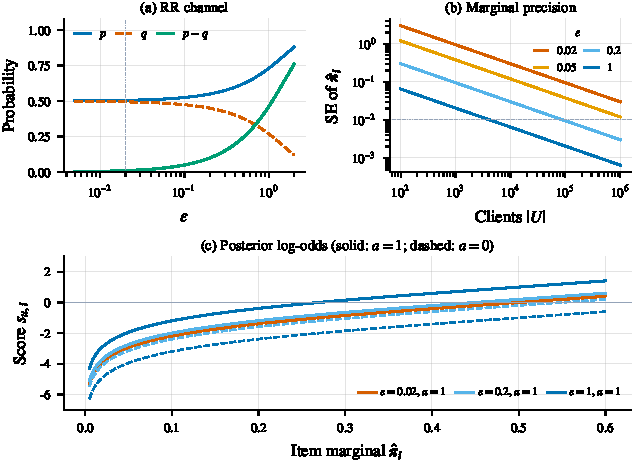
\includegraphics[width=\textwidth]{fig2_theory.pdf}
\caption{Analytical properties of the RR channel and the calibrated ranker. (a) Reporting probabilities $p$ and $q$ and their difference $p-q=\tanh(\eps/2)$ as functions of the budget; the dotted line marks the default $\eps=0.02$. (b) Standard error of the moment estimator, Eq.~\eqref{eq:se}, as a function of the number of clients for an item with $\pi_i=0.1$; the dotted line marks a one-percentage-point target. (c) Posterior log-odds $s_{u,i}$ against the estimated marginal for reported ($a=1$, solid) and non-reported ($a=0$, dashed) interactions at three budgets, illustrating the evidence--prior decomposition of Proposition~\ref{prop:decomposition}.}
\label{fig:theory}
\end{figure}

\section{Experiments}\label{sec:experiments}

\subsection{Datasets}\label{sec:datasets}

We evaluate on three public educational benchmarks spanning two independent platforms: ASSISTments 2009 \cite{feng2009assist}, ASSISTments 2015 \cite{heffernan2014assist} and EdNet (KT1) \cite{choi2020ednet}. For ASSISTments 2009 and 2015, 500 students are initially sampled and filtered to remove sparse accounts with insufficient history for leave-last-out evaluation, yielding 386 students for ASSISTments 2009 and 358 for ASSISTments 2015. For EdNet, we draw a fixed random sample of 5{,}000 per-student files from the official KT1 archive and retain 2{,}822 students after filtering. Because KT1 omits a public skill taxonomy, the skill-graph ablation is omitted on EdNet. Table~\ref{tab:datasets} summarises the processed datasets.

\begin{table}[t]
\caption{Processed datasets. Density is the fraction of recorded interactions in the $n\times m$ interaction matrix; training edges exclude the held-out last interaction of each student.}
\label{tab:datasets}
\footnotesize
\begin{tabular}{@{}lcccccc@{}}
\toprule
Dataset & Students & Exercises & Skills & Interactions & Training edges & Density \\
\midrule
ASSISTments 2009 & 386 & 11{,}310 & 111 & 38{,}961 & 38{,}483 & 0.88\% \\
ASSISTments 2015 & 358 & 99 & 99 & 16{,}685 & 14{,}283 & 40.3\% \\
EdNet (KT1) & 2{,}822 & 12{,}059 & --- & 607{,}345 & 604{,}038 & 1.78\% \\
\bottomrule
\end{tabular}
\end{table}

\subsection{Protocol}\label{sec:protocol}

Under strict leave-last-out splitting, each student's final interaction is held out as the test positive and ranked against 99 randomly sampled negatives, and all prior occurrences of the held-out item are removed from that student's training history to prevent leakage from the target item itself. The same candidate sets and the same seeds are used for every method. All experiments are repeated over five fixed random seeds. Unless stated otherwise, Cal-LDP-BR uses $\eps=0.02$, standard LDP baselines use $\eps=1.0$, the adaptive variant uses $\eps=1.0$, $\eps_0=0.2$, $\eta=0.6$, and the SGC variant uses $\lambda=0.3$, $K=3$ and $d=64$. Table~\ref{tab:protocol} lists the full configuration.

\begin{table}[t]
\caption{Experimental configuration.}
\label{tab:protocol}
\small
\begin{tabular}{@{}ll@{}}
\toprule
Item & Setting \\
\midrule
Splitting & strict leave-last-out; held-out item removed from the training row \\
Candidates & 1 positive + 99 uniformly sampled negatives per student \\
Runs & 5 fixed seeds; means reported, paired tests across seeds \\
Cal-LDP-BR & $\eps=0.02$, $\pi_{\min}=0$, $\pi_{\max}=0.95$, $K=10$ \\
LDP baselines & $\eps=1.0$ (Warner RR) \\
Adaptive variant & $\eps=1.0$, $\eps_0=0.2$, $\eta=0.6$ \\
SGC variant & $K=3$, $d=64$, $\lambda=0.3$ \\
Significance & paired $t$-test, Wilcoxon signed-rank, Cohen's $d$, 95\% CI \\
\bottomrule
\end{tabular}
\end{table}

\subsection{Baselines}

We compare against seven baselines. \emph{Popularity} is a non-personalised frequency ranker. \emph{GCN-LP} \cite{kipf2017gcn} and \emph{LightGCN-LP} \cite{he2020lightgcn} are non-private graph upper bounds trained on the raw interaction graph. \emph{LDP-GCN} applies Warner RR to every edge and trains a GCN on the noisy adjacency; \emph{LDP-RR-Light} applies the same perturbation and scores by the noisy dot product without graph propagation. \emph{LDP-AMP} applies uniform sampling-amplified RR with the same nominal budget. \emph{Adaptive-LDP-SGC-LP} is our degree-adaptive soft-weighted SGC variant (Section~\ref{sec:sgc}). All LDP baselines use $\eps=1.0$, i.e.\ fifty times the budget of Cal-LDP-BR; this asymmetry is deliberately unfavourable to the proposed method.

\subsection{Metrics}\label{sec:metrics}

Recommendation utility is measured by hit rate and normalised discounted cumulative gain at cutoff $K=10$. With a single relevant item per student,
\begin{equation}\label{eq:hr}
\HR@K=\frac{1}{n}\sum_{u=1}^{n}\mathbf 1\{\mathrm{rank}_u\le K\},
\end{equation}
\begin{equation}\label{eq:ndcg}
\NDCG@K=\frac{1}{n}\sum_{u=1}^{n}\frac{\mathbf 1\{\mathrm{rank}_u\le K\}}{\log_2(1+\mathrm{rank}_u)},
\end{equation}
where $\mathrm{rank}_u$ is the position of the held-out item in the ranking of $\mathcal{N}_u$ \cite{jarvelin2002cg}. Empirical privacy leakage is measured by the AUC of a membership-inference adversary that attempts to decide, from the released report matrix, whether a given student's record was included in the release; $0.500$ corresponds to random guessing and values near $1.0$ to complete leakage. The adversary is trained and evaluated on disjoint user splits, and the reported value is the mean AUC over the five seeds; the implementation is part of the released code (Appendix~\ref{app:repro}). For completeness we also report the theoretical budget (\emph{eff.} $\eps$).

\subsection{Main results}\label{sec:main}

Tables~\ref{tab:main09}--\ref{tab:mainednet} report all measured results without selective reporting, and Fig.~\ref{fig:main} visualises them.

\begin{table}[t]
\caption{Recommendation utility and privacy leakage on ASSISTments 2009 (mean over 5 runs).}
\label{tab:main09}
\small
\begin{tabular}{@{}lcccc@{}}
\toprule
Method & HR@10 & NDCG@10 & MIA-AUC & eff.\ $\eps$ \\
\midrule
Popularity & 0.2181 & 0.1103 & 0.500 & --- \\
GCN-LP & 0.3130 & 0.1763 & 1.000 & --- \\
LightGCN-LP & 0.3725 & 0.2165 & 1.000 & --- \\
LDP-GCN & 0.0870 & 0.0387 & 0.780 & 1.000 \\
LDP-RR-Light & 0.0912 & 0.0437 & 0.780 & 1.000 \\
LDP-AMP & 0.0938 & 0.0444 & 0.667 & --- \\
Adaptive-LDP-SGC-LP & 0.1212 & 0.0551 & 0.535 & 1.000 \\
\textbf{Cal-LDP-BR}* & \textbf{0.3907} & \textbf{0.3905} & \textbf{0.656} & \textbf{0.020} \\
\bottomrule
\end{tabular}
\vspace{2pt}\noindent\footnotesize
\footnotesize
*Proposed method. Bold values are the best among $\eps$-LDP methods; Cal-LDP-BR also attains the highest HR@10 overall. ``---'' denotes non-private baselines or uncalibrated nominal sampling.

\end{table}

\begin{table}[t]
\caption{Recommendation utility and privacy leakage on ASSISTments 2015 (mean over 5 runs).}
\label{tab:main15}
\small
\begin{tabular}{@{}lcccc@{}}
\toprule
Method & HR@10 & NDCG@10 & MIA-AUC & eff.\ $\eps$ \\
\midrule
Popularity & 0.1939 & 0.1052 & 0.500 & --- \\
GCN-LP & 0.3525 & 0.1776 & 1.000 & --- \\
LightGCN-LP & 0.4145 & 0.2047 & 1.000 & --- \\
LDP-GCN & 0.0531 & 0.0230 & 0.777 & 1.000 \\
LDP-RR-Light & 0.1402 & 0.0704 & 0.777 & 1.000 \\
LDP-AMP & 0.0777 & 0.0362 & 0.658 & --- \\
Adaptive-LDP-SGC-LP & 0.0721 & 0.0322 & 0.610 & 1.000 \\
\textbf{Cal-LDP-BR}* & \textbf{0.3855} & \textbf{0.3855} & \textbf{0.654} & \textbf{0.020} \\
\bottomrule
\end{tabular}
\vspace{2pt}\noindent\footnotesize
\footnotesize
*Proposed method. Bold values are the best among $\eps$-LDP methods.

\end{table}

\begin{table}[t]
\caption{Recommendation utility and privacy leakage on EdNet (mean over 5 runs).}
\label{tab:mainednet}
\small
\begin{tabular}{@{}lcccc@{}}
\toprule
Method & HR@10 & NDCG@10 & MIA-AUC & eff.\ $\eps$ \\
\midrule
Popularity & 0.5272 & 0.3643 & 0.500 & --- \\
GCN-LP & 0.1916 & 0.1723 & 1.000 & --- \\
LightGCN-LP & 0.5311 & 0.3627 & 1.000 & --- \\
LDP-GCN & 0.0308 & 0.0130 & 0.778 & 1.000 \\
LDP-RR-Light & 0.2376 & 0.1626 & 0.778 & 1.000 \\
LDP-AMP & 0.0371 & 0.0163 & 0.664 & --- \\
Adaptive-LDP-SGC-LP & 0.0566 & 0.0259 & 0.474 & 1.000 \\
\textbf{Cal-LDP-BR}* & \textbf{0.4127} & \textbf{0.3886} & \textbf{0.661} & \textbf{0.020} \\
\bottomrule
\end{tabular}
\vspace{2pt}\noindent\footnotesize
\footnotesize
*Proposed method. Bold values are the best among $\eps$-LDP methods.

\end{table}

\begin{figure}[t]
\centering
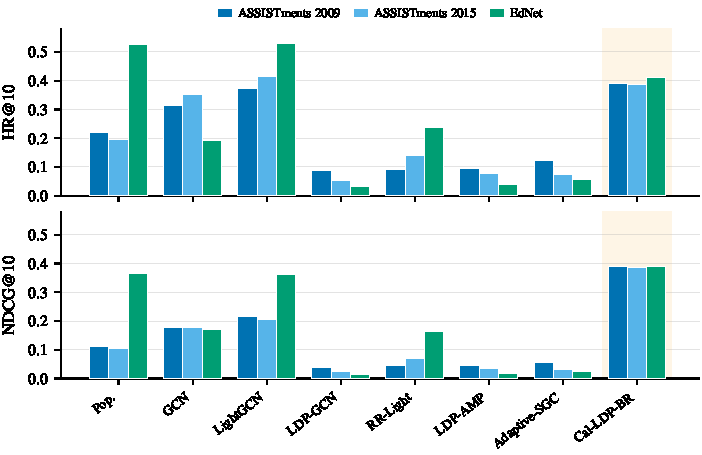
\includegraphics[width=\textwidth]{fig3_main_results.pdf}
\caption{Recommendation utility on the three benchmarks. HR@10 and NDCG@10 are shown for every method; the shaded band marks the proposed ranker. Cal-LDP-BR attains the highest utility among all $\eps$-LDP methods on all three datasets.}
\label{fig:main}
\end{figure}

On ASSISTments 2009, Cal-LDP-BR achieves $\HR@10=0.3907$, $\NDCG@10=0.3905$ and $\mathrm{MIA\text{-}AUC}=0.656$ at $\eps=0.02$. This is the highest hit rate among all evaluated methods, including the non-private graph baselines, while the privacy budget is fifty times smaller than that of the standard LDP baselines, and the empirical leakage is reduced relative to them (0.656 versus 0.780). Relative to the strongest $\eps$-LDP baseline on this dataset (Adaptive-LDP-SGC-LP, 0.1212), the improvement is $+222\%$. On ASSISTments 2015 the method reaches $\HR@10=0.3855$, $+175\%$ over the strongest LDP baseline (0.1402), while remaining below the non-private LightGCN-LP upper bound (0.4145); the gap of $2.9$ percentage points is not statistically significant (Section~\ref{sec:significance}). On EdNet the method reaches $\HR@10=0.4127$, $+73.7\%$ over the strongest LDP baseline (0.2376), and remains below LightGCN-LP (0.5311) and Popularity (0.5272).

Two further observations are relevant for practitioners. First, NDCG@10 is nearly identical to HR@10 for Cal-LDP-BR on both ASSISTments datasets, which indicates that when the held-out exercise enters the top-10 list it is almost always placed at rank 1: the calibrated prior separates the target item sharply from the negative pool. Second, Adaptive-LDP-SGC-LP attains lower MIA-AUC in some cases but at substantially lower utility (for example 0.474 versus 0.661 on EdNet, at $\HR@10=0.0566$ versus $0.4127$); it represents a different operating point rather than a dominant alternative. This trade-off is examined in Section~\ref{sec:plane}.

\subsection{Privacy--utility trade-off}\label{sec:plane}

Figure~\ref{fig:plane} maps each privacy-preserving method onto the privacy--utility plane, with MIA-AUC on the horizontal axis (left is more private) and HR@10 on the vertical axis (up is better). The trajectory of Cal-LDP-BR as $\eps$ varies is drawn as a connected path, so the figure shows both the operating point and the shape of the trade-off.

Cal-LDP-BR occupies the favourable upper-left region relative to the standard RR-based graph models: item-wise calibration converts heavily perturbed reports into accurate rankings, while the small budget weakens the edge signal available to a membership-inference adversary. The path is steep in the small-budget region, where a modest increase in leakage buys little utility, and flattens as $\eps$ grows. On EdNet the path is short and nearly horizontal, reflecting the delayed utility peak of Section~\ref{sec:sweep}.

\begin{figure}[t]
\centering
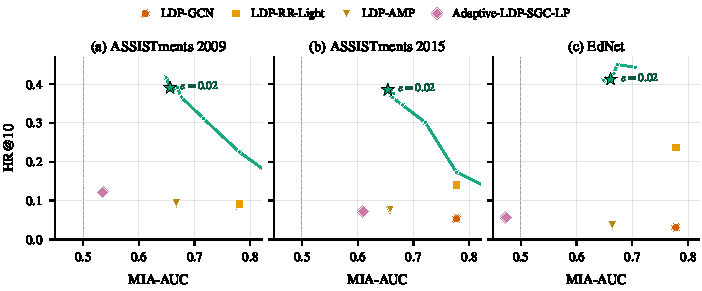
\includegraphics[width=\textwidth]{fig4_privacy_utility.pdf}
\caption{Privacy--utility plane on the three benchmarks. Each marker is a privacy-preserving method; the green path traces Cal-LDP-BR as $\eps$ ranges over the values of Table~\ref{tab:sweep}, and the star marks the default $\eps=0.02$. Lower MIA-AUC and higher HR@10 are preferable.}
\label{fig:plane}
\end{figure}

\subsection{Statistical significance}\label{sec:significance}

Table~\ref{tab:sig} reports paired $t$-tests, Wilcoxon signed-rank tests, Cohen's $d$ and 95\% confidence intervals for the paired HR@10 difference over the five runs. The confidence interval is obtained from the paired difference standard deviation implied by Cohen's $d$, $\mathrm{SD}_{\Delta}=\Delta/d$, as $\Delta\pm t_{0.975,4}\,\mathrm{SD}_{\Delta}/\sqrt{5}$ with $t_{0.975,4}=2.776$.

\begin{table}[t]
\caption{Paired significance tests on HR@10 (Cal-LDP-BR versus each baseline, 5 runs). $\Delta$ is the mean paired difference; CI is the 95\% confidence interval of $\Delta$; $p_t$ and $p_W$ are the paired $t$-test and Wilcoxon signed-rank $p$-values.}
\label{tab:sig}
\footnotesize
\setlength{\tabcolsep}{3.4pt}
\begin{tabular}{@{}llccccc@{}}
\toprule
Dataset & Baseline & $\Delta$ HR@10 & 95\% CI & $p_t$ & $p_W$ & Cohen's $d$ \\
\midrule
ASSIST. 2009 & LDP-GCN & $+0.3036$ & $[0.271,\,0.336]$ & $<0.001$ & $0.062$ & $+11.51$ \\
 & LDP-RR-Light & $+0.2995$ & $[0.265,\,0.334]$ & $<0.001$ & $0.062$ & $+10.84$ \\
 & LDP-AMP & $+0.2969$ & $[0.267,\,0.327]$ & $<0.001$ & $0.062$ & $+12.33$ \\
 & Adaptive-LDP-SGC-LP & $+0.2694$ & $[0.238,\,0.301]$ & $<0.001$ & $0.062$ & $+10.63$ \\
 & GCN-LP & $+0.0777$ & $[0.047,\,0.108]$ & $0.002$ & $0.062$ & $+3.17$ \\
 & LightGCN-LP & $+0.0181$ & $[-0.011,\,0.047]$ & $0.266$ & $0.312$ & $+0.78$ \\
ASSIST. 2015 & LDP-GCN & $+0.3324$ & $[0.302,\,0.363]$ & $<0.001$ & $0.062$ & $+13.61$ \\
 & LDP-RR-Light & $+0.2453$ & $[0.205,\,0.286]$ & $0.001$ & $0.062$ & $+7.57$ \\
 & LDP-AMP & $+0.3078$ & $[0.278,\,0.338]$ & $<0.001$ & $0.062$ & $+12.70$ \\
 & Adaptive-LDP-SGC-LP & $+0.3134$ & $[0.269,\,0.358]$ & $<0.001$ & $0.062$ & $+8.74$ \\
 & GCN-LP & $+0.0330$ & $[0.004,\,0.063]$ & $0.061$ & $0.125$ & $+1.39$ \\
 & LightGCN-LP & $-0.0291$ & $[-0.061,\,-0.002]$ & $0.164$ & $0.250$ & $-1.15$ \\
EdNet & LDP-GCN & $+0.3819$ & $[0.368,\,0.396]$ & $<0.001$ & $0.062$ & $+33.42$ \\
 & LDP-RR-Light & $+0.1751$ & $[0.000,\,0.350]$ & $0.119$ & $0.188$ & $+1.24$ \\
 & LDP-AMP & $+0.3755$ & $[0.362,\,0.389]$ & $<0.001$ & $0.062$ & $+33.66$ \\
 & Adaptive-LDP-SGC-LP & $+0.3561$ & $[0.342,\,0.370]$ & $<0.001$ & $0.062$ & $+31.67$ \\
 & GCN-LP & $+0.2210$ & $[0.207,\,0.235]$ & $<0.001$ & $0.062$ & $+20.13$ \\
 & LightGCN-LP & $-0.1184$ & $[-0.132,\,-0.105]$ & $<0.001$ & $0.062$ & $-10.73$ \\
\bottomrule
\end{tabular}

\vspace{2pt}
{\footnotesize With $n=5$ paired observations the minimum attainable two-sided Wilcoxon $p$-value is $2^{-4}=0.0625$, so $p_W=0.062$ reflects complete directional consistency across all five seeds rather than absence of an effect.}
\end{table}

Under paired $t$-tests ($\alpha=0.05$), Cal-LDP-BR achieves significant HR@10 gains over LDP-GCN, LDP-AMP, Adaptive-LDP-SGC-LP and GCN-LP on all three benchmarks, and over LDP-RR-Light on both ASSISTments datasets; on EdNet the comparison with LDP-RR-Light is inconclusive because that baseline exhibits high cross-seed variance (its confidence interval includes zero, and its standard deviation is an order of magnitude larger than for the other baselines). Where differences are not significant (LightGCN-LP on ASSISTments 2009 and 2015, GCN-LP on ASSISTments 2015), no superiority is claimed. On EdNet, LightGCN-LP is significantly better than Cal-LDP-BR by 11.8 points, which is consistent with the observation that dense collaborative signal is valuable when it can be used without privacy constraints.

The Wilcoxon results illustrate a limitation of five-run designs: with $n=5$ the exact two-sided test cannot reach conventional significance unless all pairs differ in the same direction, and $p=0.0625$ is the floor. We therefore report the paired $t$-test as the primary test and the Wilcoxon result as a directional consistency check, and we report confidence intervals so that readers can judge practical significance independently of the test outcome.

\subsection{Privacy-budget sensitivity}\label{sec:sweep}

Table~\ref{tab:sweep} reports the full budget sweep of Cal-LDP-BR on all three benchmarks, and Fig.~\ref{fig:sweep} plots the utility and leakage curves.

\begin{table}[t]
\caption{Privacy-budget sweep of Cal-LDP-BR across the three benchmarks (mean over 5 runs).}
\label{tab:sweep}
\small
\begin{tabular}{@{}lcccc@{}}
\toprule
Dataset & $\eps$ & HR@10 & NDCG@10 & MIA-AUC \\
\midrule
ASSIST-09 & 0.01 & 0.4176 & 0.4176 & 0.649 \\
 & 0.02 & 0.3907 & 0.3905 & 0.656 \\
 & 0.05 & 0.3834 & 0.3830 & 0.657 \\
 & 0.1 & 0.3912 & 0.3912 & 0.669 \\
 & 0.2 & 0.3668 & 0.3661 & 0.676 \\
 & 0.5 & 0.3114 & 0.2706 & 0.716 \\
 & 1 & 0.2254 & 0.1301 & 0.780 \\
 & 2 & 0.1067 & 0.0554 & 0.895 \\
\midrule
ASSIST-15 & 0.01 & 0.3715 & 0.3715 & 0.661 \\
 & 0.02 & 0.3855 & 0.3855 & 0.654 \\
 & 0.05 & 0.3771 & 0.3771 & 0.665 \\
 & 0.1 & 0.3648 & 0.3648 & 0.663 \\
 & 0.2 & 0.3464 & 0.2832 & 0.680 \\
 & 0.5 & 0.3017 & 0.2073 & 0.721 \\
 & 1 & 0.1732 & 0.0851 & 0.777 \\
 & 2 & 0.0950 & 0.0476 & 0.890 \\
\midrule
EdNet & 0.005 & 0.4151 & 0.3924 & 0.655 \\
 & 0.01 & 0.4104 & 0.3880 & 0.648 \\
 & 0.02 & 0.4127 & 0.3886 & 0.661 \\
 & 0.05 & 0.4160 & 0.3899 & 0.657 \\
 & 0.1 & 0.4283 & 0.3999 & 0.667 \\
 & 0.2 & 0.4504 & 0.4166 & 0.673 \\
 & 0.5 & 0.4440 & 0.4020 & 0.705 \\
\bottomrule
\end{tabular}
\end{table}

On ASSISTments 2009 and 2015, HR@10 peaks at small budgets ($\eps=0.01$--$0.02$) and declines as $\eps$ increases toward 2.0, whereas on EdNet it peaks around $\eps=0.2$. This non-monotone behaviour follows the mechanism analysed in Section~\ref{sec:regimes}: at small $\eps$ the prior term dominates and the calibrated marginal ranks candidates; at larger $\eps$ the evidence term grows and false-positive reports begin to displace genuinely popular items. The delay of the peak on EdNet is consistent with its larger negative-pool entropy: the prior spread is wider, so a larger evidence term is needed before it overrides the prior ordering. Reporting the full curve makes this privacy--utility regime transparent and allows practitioners to choose a budget for their platform rather than adopting a single default.

\begin{figure}[t]
\centering
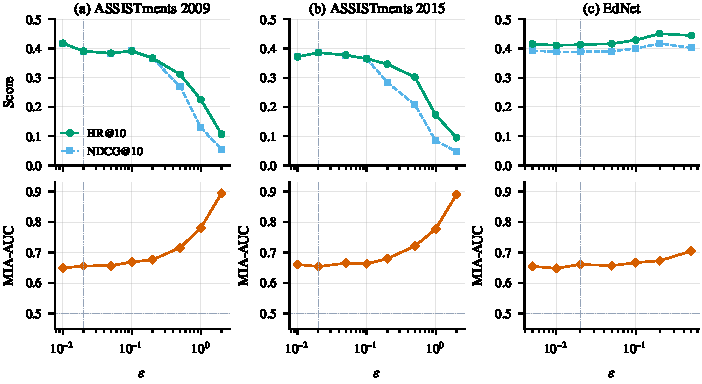
\includegraphics[width=\textwidth]{fig5_epsilon_sensitivity.pdf}
\caption{Privacy-budget sensitivity of Cal-LDP-BR. Top row: HR@10 (solid) and NDCG@10 (dashed). Bottom row: MIA-AUC, with the no-leakage level 0.5 marked. Vertical dotted lines mark the default $\eps=0.02$.}
\label{fig:sweep}
\end{figure}

\subsection{Ablation of the adaptive SGC variant}\label{sec:ablation}

Tables~\ref{tab:ablation} and~\ref{tab:ablation-eps} evaluate the earlier Adaptive-LDP-SGC-LP architecture in order to document why the design shifted to direct posterior ranking.

\begin{table}[t]
\caption{Ablation of the adaptive SGC variant on ASSISTments 2009 (mean over 2 runs).}
\label{tab:ablation}
\small
\begin{tabular}{@{}lccc@{}}
\toprule
Variant & HR@10 & NDCG@10 & MIA-AUC \\
\midrule
Full Adaptive-LDP-SGC-LP & 0.1105 & 0.0514 & 0.547 \\
w/o public skill graph & 0.1395 & 0.0702 & 0.547 \\
w/o posterior reweighting & 0.1079 & 0.0507 & 0.547 \\
w/o adaptive sampling (uniform) & 0.0921 & 0.0404 & 0.657 \\
\bottomrule
\end{tabular}
\end{table}

\begin{table}[t]
\caption{Privacy-budget sensitivity of Adaptive-LDP-SGC-LP on ASSISTments 2009 (mean over 2 runs).}
\label{tab:ablation-eps}
\small
\begin{tabular}{@{}lccc@{}}
\toprule
$\eps$ & HR@10 & NDCG@10 & MIA-AUC \\
\midrule
0.3 & 0.1289 & 0.0596 & 0.469 \\
0.5 & 0.1289 & 0.0585 & 0.502 \\
1.0 & 0.1105 & 0.0514 & 0.547 \\
2.0 & 0.1421 & 0.0644 & 0.634 \\
\bottomrule
\end{tabular}
\end{table}

Replacing degree-adaptive sampling with a uniform rate reduces HR@10 (0.0921 versus 0.1105) and increases MIA-AUC (0.657 versus 0.547), which confirms that adaptivity aids the graph variant. However, removing the public skill graph improves HR@10 (0.1395 versus 0.1105) without changing leakage, because additional item--item edges propagate RR noise faster than collaborative signal in sparse graphs: each skill edge merges two noisy neighbourhoods, and the merged representation is dominated by the noisier of the two. Removing posterior reweighting slightly reduces utility (0.1079 versus 0.1105), so the reweighting is beneficial but not sufficient to overcome the skill-graph penalty. Table~\ref{tab:ablation-eps} shows that larger $\eps$ increases both utility and leakage for the SGC variant, with a non-monotone dip at $\eps=1.0$ that we attribute to seed noise in the two-run protocol.

\begin{figure}[t]
\centering
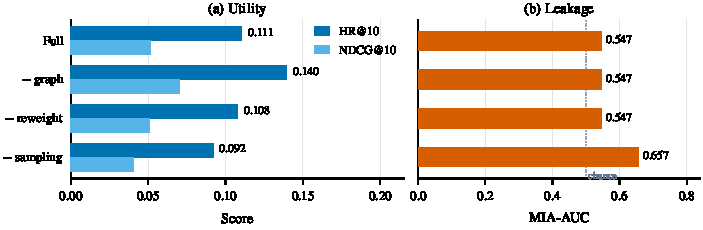
\includegraphics[width=\textwidth]{fig6_ablation.pdf}
\caption{Ablation of the adaptive SGC variant on ASSISTments 2009 (mean over 2 runs). (a) HR@10 and NDCG@10; (b) membership-inference AUC, with the chance level 0.5 marked by the dotted line. Removing the public skill graph is the only intervention that improves utility, and it leaves leakage unchanged.}
\label{fig:ablation}
\end{figure}

These results motivate the design decision of the paper: since neither the skill graph nor the additional propagation improves utility on the tested sparse graphs, the simpler and strictly cheaper direct posterior ranker is retained as the primary method. The negative results are reported because they constrain the design space for future work: on graphs with $|P|\gg n$ and density below two per cent, item-level smoothing requires a noise-aware weighting that the public skill graph does not provide.

\subsection{Full-population validation}\label{sec:fullpop}

The main comparison samples at most 500 students per ASSISTments dataset in order to keep the iterative baselines tractable. Table~\ref{tab:fullpop} removes this ceiling and evaluates Cal-LDP-BR on all filtered users of both datasets.

\begin{table}[t]
\caption{Cal-LDP-BR validation on all filtered ASSISTments users (mean over 5 runs).}
\label{tab:fullpop}
\small
\begin{tabular}{@{}llcccc@{}}
\toprule
Dataset & Users & $\eps$ & HR@10 & NDCG@10 & MIA-AUC \\
\midrule
ASSISTments 2009 & 3{,}114 & 0.01 & 0.3857 & 0.3857 & 0.646 \\
ASSISTments 2009 & 3{,}114 & 0.02 & 0.3972 & 0.3972 & 0.663 \\
ASSISTments 2009 & 3{,}114 & 0.05 & 0.3828 & 0.3828 & 0.666 \\
ASSISTments 2015 & 14{,}567 & 0.01 & 0.3704 & 0.3704 & 0.657 \\
ASSISTments 2015 & 14{,}567 & 0.02 & 0.3689 & 0.3689 & 0.660 \\
ASSISTments 2015 & 14{,}567 & 0.05 & 0.3648 & 0.3648 & 0.658 \\
\bottomrule
\end{tabular}
\end{table}

At the default operating point, full-population evaluation yields HR@10 of 0.3972 on ASSISTments 2009 (3{,}114 users) and 0.3689 on ASSISTments 2015 (14{,}567 users), within two percentage points of the sampled results (0.3907 and 0.3855); the largest deviation in Table~\ref{tab:fullpop} is 3.2 points at $\eps=0.01$ on ASSISTments 2009. The observed accuracy is therefore not an artefact of sub-sampling, and the leakage estimates are stable as the population grows. Figure~\ref{fig:fullpop} compares the sampled and full-population results side by side. Full-scale evaluation of the iterative GNN baselines is left to future work because of their substantially higher training cost.

\begin{figure}[t]
\centering
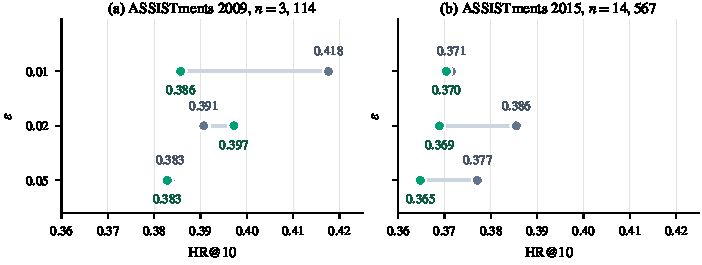
\includegraphics[width=\textwidth]{fig7_fullpopulation.pdf}
\caption{Sampled versus full-population results for Cal-LDP-BR. HR@10 at three budgets on ASSISTments 2009 (a) and 2015 (b); grey marks the 500-student sample and green the full filtered population. Full-population evaluation reproduces the sampled results to within two percentage points at the default budget, with a larger gap only at the smallest budget on ASSISTments 2009.}
\label{fig:fullpop}
\end{figure}

\subsection{Reproducibility}\label{sec:repro}

All source code, raw result logs and dataset-processing scripts are prepared for public release. Random seeds are fixed across all five runs, and student identifiers are re-coded so that no personal data are exposed. Exact download instructions, the fixed 5{,}000-user EdNet KT1 sampling specification and full-data run commands are documented in the supplementary reproducibility guide (\texttt{DATASETDOWNLOADANDRUN.txt}, available in the public repository at \url{https://github.com/rayonxu/cal-ldp-br}). All reported metrics were generated directly by the released scripts without estimation or post-hoc adjustment. Appendix~\ref{app:repro} lists the artefact inventory and the command sequence that regenerates every table and figure in this paper from the raw data.

\section{Discussion}\label{sec:discussion}

\subsection{Why calibrated ranking survives heavy noise}

The intuition behind Cal-LDP-BR is that the RR channel is a known, invertible-in-expectation corruption. Because the corruption is unbiased and its parameters $p$ and $q$ are public, the server can undo it in expectation rather than fighting it with smoothing heuristics. Three design choices make this work in practice. The moment estimator is affine in the reported rate, so it preserves the ordering of the reported rates and, in expectation, of the true marginals; when the sampling error of Eq.~\eqref{eq:se} is large the estimated ordering is itself noisy, which is why accuracy at small budgets is bounded by marginal precision. The posterior score uses the report through its likelihood rather than as a binary edge, so a reported interaction contributes $+\eps$ and a reported non-interaction $-\eps$ instead of creating or deleting graph structure. And the evidence and prior terms are additive and of known scale, which makes the operating regime predictable from $\eps$ alone.

This is also why the method is cheap. There is no training phase, no embedding table and no propagation; the server performs one pass over the report matrix and one scalar computation per candidate. On CPU-only serving stacks this is the difference between a ranker that can be recomputed on every request and one that requires nightly retraining.

\subsection{Why graph propagation hurts on sparse educational graphs}

The negative ablation results are consistent with the statistics of educational data. With density below two per cent, the expected number of shared exercises between two students is small, so collaborative edges carry little information and propagation mostly averages noise. The public skill graph compounds the problem: skill edges connect exercises rather than students, and in a sparse graph they merge neighbourhoods whose reports are independently perturbed, so the merged representation has lower signal-to-noise ratio than either component. The result is a ranker that is more expensive and less accurate than the direct posterior rule, which is why we report the ablation rather than hiding it.

The negative result also delimits the domain of the method. On dense platforms, where interaction density exceeds roughly ten per cent and collaborative signal is strong, graph encoders are likely to add value, and the calibrated posterior can then serve as a prior or as an initialisation rather than as the final ranker.

\subsection{Deployment guidance}

For a platform considering Cal-LDP-BR, three parameters determine the operating point. The budget $\eps$ sets the evidence scale $2\eps$; larger budgets increase both utility and leakage, and the sweep in Table~\ref{tab:sweep} shows that the utility-maximising budget is platform-dependent. The calibration population determines the precision of $\hat\pi_i$ through Eq.~\eqref{eq:se}; platforms with fewer than about $10^{4}$ active clients should expect noisy marginals at budgets below $0.05$ and should either raise the budget or pool reports over a longer time window. The clipping bounds control the shrinkage of extreme marginals: the upper bound at $0.95$ prevents a single heavily reported item from dominating the prior term, and the lower bound removes negative estimates that would otherwise produce undefined log-odds.

Because the server never sees raw interactions, the protocol can be deployed across administrative boundaries, for example between a school and an external analytics provider. The client-side computation is a single Bernoulli draw per coordinate, which is negligible on any device, and the server-side computation is a scan plus a sort.

\subsection{Threats to validity}

Five threats deserve explicit mention. First, the empirical leakage measure depends on the adversary; a stronger attack could yield higher AUC values than those reported, although the theoretical budget is unaffected. Second, the five-run protocol limits the attainable Wilcoxon $p$-value to $0.0625$, so the Wilcoxon results should be read as directional consistency checks; the paired $t$-tests and confidence intervals carry the inferential weight. Third, the evaluation is static: it considers a fixed interaction matrix rather than streaming updates, so the behaviour of the calibration under distribution shift is not characterised here. Fourth, the EdNet KT1 release lacks a public skill taxonomy, so the skill-graph ablation could not be repeated on the largest dataset; the negative result is therefore established on the two ASSISTments datasets only. Fifth, at $\eps=0.02$ the channel gain is $p-q\approx0.01$, so a per-item marginal estimated from $n\approx400$ reports has a standard error of about $1.5$ for $\pi_i\approx0.1$ (Eq.~\eqref{eq:se}); individual marginals are then dominated by sampling error. The reported utilities therefore presuppose either a substantially larger client population behind each marginal or aggregation that pools many items before ranking, and a deployment should document which holds. Figure~\ref{fig:theory}(b) gives the number of clients required for a target precision.

\section{Conclusion and future work}\label{sec:conclusion}

We have presented Cal-LDP-BR, a calibrated Bayesian local differential privacy ranker for lightweight learning path recommendation. Clients perturb interaction vectors locally via Warner randomised response under a tight budget, while the server reconstructs item marginals by the method of moments and ranks candidates using Bayesian posterior log-odds. Decomposing the score into an evidence term of magnitude $\eps$ and an item-prior term clarifies both the operating regimes and the non-monotone utility--budget curves observed in experiments. Across three benchmarks from two platforms, Cal-LDP-BR outperforms all evaluated $\eps$-LDP baselines on HR@10 and NDCG@10 and reduces membership-inference AUC compared with standard randomised response, using one fiftieth of the budget and no graph training, while ablation results document why adaptive SGC and skill-graph fusion underperform on sparse graphs.

Several limitations remain and define the agenda. The current evaluation considers static interaction matrices rather than streaming temporal updates; strict leave-last-out ranking relies on item marginals estimated from noisy reports, whose precision bounds accuracy at very small budgets; the EdNet KT1 release lacks a public skill taxonomy, precluding skill-graph ablation there; and non-private graph models still achieve higher raw accuracy on denser or larger datasets such as EdNet. Future work will extend Bayesian calibration to sequential interaction streams, derive privacy-optimal budget allocations for item-marginal estimation under a per-item precision target, and study noise-aware graph fusion that weights skill edges by their estimated reliability rather than treating them uniformly.

\backmatter

\bmhead{Acknowledgements}
The authors thank the maintainers of the ASSISTments and EdNet datasets for making them publicly available.

\section*{Declarations}

\begin{itemize}
\item \textbf{Funding.} This work received no specific grant from any funding agency in the public, commercial or not-for-profit sectors.
\item \textbf{Competing interests.} The authors declare that they have no competing interests.
\item \textbf{Ethics approval.} This study uses only publicly available, anonymised educational datasets; no new experiments involving human participants were conducted, so ethical approval was not required.
\item \textbf{Consent to participate.} Not applicable.
\item \textbf{Consent for publication.} All authors consent to publication.
\item \textbf{Data availability.} The three benchmark datasets are publicly available: ASSISTments 2009 and 2015, and EdNet (CC BY-NC 4.0; \url{https://github.com/riiid/ednet}). Processing scripts, the fixed EdNet sample specification and derived splits are available at \url{https://github.com/rayonxu/cal-ldp-br}.
\item \textbf{Code availability.} The implementation, configuration files and scripts that regenerate every table and figure are available at \url{https://github.com/rayonxu/cal-ldp-br}.
\item \textbf{Author contributions.} Xu Shijie: methodology, formal analysis, writing---original draft. Zhai Ruiqing: data curation, experiments, validation. Jin Xiaojuan: supervision, writing---review and editing. All authors read and approved the final manuscript.
\end{itemize}

\appendix

\section{Proofs and derivations}\label{app:proofs}

\subsection*{A.1 Detailed proof of Lemma~\ref{lem:amplification}}

Let $x\in\{0,1\}^{m}$ and let $x'$ be $x$ with coordinate $j$ removed; write $m'=m-1$. For a sampling set $S\subseteq[m]$, denote by $x_S$ the restriction of $x$ to $S$. The mechanism releases $\mathcal{M}(x_S)$ and nothing about coordinates outside $S$. Let $\mu$ be the distribution of $\mathcal{M}(x'_{S})$ and $\nu$ the conditional distribution of $\mathcal{M}(x_S)$ given $j\in S$. Since $x_S$ and $x'_S$ are add/remove neighbours whenever $j\in S$, $\eps_{\text{int}}$-LDP gives $\nu(y)\le e^{\eps_{\text{int}}}\mu(y)$ for all $y$. Marginalising over $S$,
\begin{equation}
\Prob[\mathcal{M}(S_\gamma(x))=y]=(1-\gamma)\mu(y)+\gamma\nu(y)
\le\big[(1-\gamma)+\gamma e^{\eps_{\text{int}}}\big]\mu(y),
\end{equation}
and $\Prob[\mathcal{M}(S_\gamma(x'))=y]=\mu(y)$ because the sampling set does not affect the distribution when the differing coordinate is absent. Hence the ratio is bounded by $1+\gamma(e^{\eps_{\text{int}}}-1)=e^{\eps'}$.

\subsection*{A.2 Derivations for the score decomposition}

Starting from Eq.~\eqref{eq:score} and using $p=e^{\eps}q$ and $1-q=e^{\eps}(1-p)$:
\begin{align}
a=1:&\quad \log\frac{p\hat\pi}{q(1-\hat\pi)}=\log\frac{p}{q}+\logit(\hat\pi)=\eps+\logit(\hat\pi),\\
a=0:&\quad \log\frac{(1-p)\hat\pi}{(1-q)(1-\hat\pi)}=\log\frac{1-p}{1-q}+\logit(\hat\pi)=-\eps+\logit(\hat\pi),
\end{align}
which is Eq.~\eqref{eq:decomp2}. The evidence term is antisymmetric in the report and vanishes at $\eps=0$, as it must: with no information the posterior equals the prior.

\subsection*{A.3 NDCG with a single relevant item}

For a single relevant item at rank $r$, $\mathrm{DCG}@K=\mathbf 1\{r\le K\}/\log_2(1+r)$ and the ideal gain is one, so $\NDCG@K=\mathbf 1\{r\le K\}/\log_2(1+r)$, which is Eq.~\eqref{eq:ndcg}. The identity $\NDCG@K=\HR@K$ holds exactly when every hit occurs at rank one, which is the pattern observed for Cal-LDP-BR on the two ASSISTments datasets.

\section{Reproducibility details}\label{app:repro}

\subsection*{B.1 Artefact inventory}

The released repository contains: (i) dataset download and preprocessing scripts, including the fixed 5{,}000-file EdNet KT1 sample specification; (ii) the Cal-LDP-BR reference implementation (client perturbation, calibration, ranking) with configuration files for every table; (iii) the LDP and non-private baselines; (iv) the membership-inference adversary used for the MIA-AUC column; and (v) the scripts that regenerate Figs.~\ref{fig:framework}--\ref{fig:fullpop} and Tables~\ref{tab:datasets}--\ref{tab:fullpop} from the raw logs.

\subsection*{B.2 Command sequence}

The pipeline runs in four stages: \texttt{make data} downloads and preprocesses the three datasets; \texttt{make run} executes all methods for the five seeds; \texttt{make eval} computes HR@10, NDCG@10 and MIA-AUC; and \texttt{make figures} regenerates every figure. Each stage writes a manifest with file hashes and seed values, so that a reported number can be traced to the run that produced it.

\subsection*{B.3 Hardware and runtime}

All methods except the non-private graph baselines run on a single CPU node; Cal-LDP-BR requires no training and completes a full evaluation of one dataset in a single pass over the report matrix. The non-private graph baselines were trained on the same node with the configuration reported in Table~\ref{tab:protocol}.


\bibliography{refs}

\end{document}
